\subsubsection{Supremum Augmented Dickey Fuller}
\label{sec:methods_features_sadf}

Section \ref{sec:intro_domain} briefly introduced the concept of structural
breaks and the index to be implemented and used in this research project, SADF.
In words of Lopez de Prado:

\say{In developing an ML-based investment strategy, we typically wish to bet
when there is a confluence of factors whose predicted outcome offers a favorable
risk-adjusted return. Structural breaks, like transition from one market regime
to another, is one example of particular interest.}

The problem appears when trying to quantitatively detect how a regime change
occurs. In \cite{sadf_paper} Phillips, Wu and Yu studied Nasdaq index in 1990
prior to the famous DotCom bubble and proposed a new index based on recursive 
augmented Dickey-Fuller tests for unit root against the alternative of an
explosive root (the right-tailed). The objective of this test is to identify
the presence of exponential growth or collapse, while assuming an autoregressive
specification.

In price series, like the one used in this research project, not only
one, but many bubbles are prune to happen. Not all indexes are useful under this
assumption as many fail to detect recurrent bubbles. Nevertheless, we will start
analyzing the case of just one bubble in the series and then generalize it to
many as the it is described in chapter 17 of \cite{lopez_de_prado}. Suppose a
price series that follows a first order autoregressive process:

\[ y_{t} = \rho y_{t-1} + \epsilon_{t} \]

where $\epsilon_{t} \sim N(0, \sigma_{y}^{2})$, i.e. white noise. We can create a
test to evaluate the value of $\rho$ whose null hypothesis states that the price
series follows a random walk. In other words, $H_{0}: \rho = 1$ and the
alternative hypothesis is that $y_t$ starts as a random walk but at some point
in time $t^{*}T$ the process becomes explosive, such:

\begin{equation}
  H_{1} :
    \begin{cases}
      \rho = 1 & \text{if t = 1, ..., $\tau^{*}T$}\\
      \rho > 1 & \text{if t = $\tau^{*}T$, ..., T}\\
    \end{cases}       
\end{equation}

where $\tau^{*} \in (0,1)$. At the end of the series, i.e. at $T$, one
could try to find the value $\tau^{*}$ where there was a change of regime from
random walk to an explosive process. To test this hypothesis, we should
consider:

\[ \Delta y_{t} = \delta y_{t-1} D_t[\tau^{*}] + \epsilon_{t}\]

where $D_t[\tau^{*}]$ is a dummy variable that takes the value of 0 when
$t < \tau^{*}T$ and 1 otherwise. $H_{0}: \delta = 0$ which is tested against the
one-sided alternative $H_{1}: \delta > 1$ leading to an statistic:

\[ DFC_{\tau^{*}} = \frac{\hat{\delta}}{\hat{\sigma}_{\delta}} \]

One needs to determine the value of $\tau^{*}$ because it is unknown. The
approach to determine it is to compute the supremum statistic for each possible
value of $\tau^{*}$ in the series. That would determine the start of the explosive
process yielding to a bubble. Note that only the beginning of the regime change
is determined with this method, i.e. there is no return to a random walk after
the bubble starts. This is where the novelty of Phillips, Wu and Yu appears by
a few key differences to the autoregressive model and test:

\begin{itemize}
  \item The regression specification becomes: $ \Delta y_t = \alpha + \beta y_{t-1} + \sum_{l=1}^{L} \gamma_{l} \Delta y_{t-l} + \epsilon_t$
  \item $H_{0}: \beta \le 0$, and $H_{1}: \beta > 0$
  \item $SADF_t = \sup_{t_{0} \in [1, t-\tau]} \{ADF_{t_{0},t}\} = \sup_{t_{0} \in [1, t-\tau]} \frac{\hat{\beta}_{t_{0},t}}{\hat{\sigma}_{\beta_{0},t}}$
\end{itemize}

A few differences with respect to the original, one-bubble model can be noted:

\begin{itemize}
  \item The regression is changed, there is no more a dummy $D_t[\tau^{*}]$
        variable. Instead, the regression starts at $t_{0} \in [1, t-\tau]$ and
        ends in $t \in [\tau, T]$.
  \item $SADF_t$ computes the supremum in a double nested loop for every
        possible value of $t_0$ and $t$ which are the indexes to segment the
        series.
\end{itemize}

The aforementioned characteristics allows SADF to vary provided that it is not
computed just for one time ($T$), but instead for many (every value of
$t \in [\tau, T]$).

Getting into the details of the augmented Dickey-Fuller statistic, the
confidence value should be set from the sample to yield the best results. In
\cite{sadf_paper} the authors refer to a value close to 4\% to deliver the best
performance but values between 1\% and 5\% are recommended. 5\% was used in this
case.

\paragraph{Implementation notes:} Lopez de Prado offers in his book almost
the entire algorithm (see chapter 17 of \cite{lopez_de_prado}), but leaves
behind the outer loop which allows to move forward the $SADF_{t}$ for each
$t \in [\tau, T]$. A modification was introduced in code to avoid excessive and
inefficient computation in the inner loop: an upper bound for the window was
introduced to so that the range of $t$ becomes $[max(\tau, t - \Delta t_{max}), T]$.
Although the asymptotic computational complexity of this series generation is
high ($O(n^5)$ at least, see \cite{lopez_de_prado} for a detailed analysis), one
way to saturate one order is to use $\Delta t_{max}$ which should be cautiously
selected to account for long lasting bubbles.

On a separate note, the algorithm allows researchers to introduce a constant, a
linear and a quadratic polynomial regression depending on the type of series to
analyze. All of them were computed in favor of feeding the model with more data
and experiment what yields the best results.

Finally, a recommendation in the article \cite{sadf_paper} and discussed in
\cite{lopez_de_prado} has been implemented. Instead of using raw prices, the
algorithm takes as input log-prices. Conceptually, by applying the logarithmic
transformation, the variance of the process gets stabilized and the
heteroscedastic assumption about the data can be fulfilled. Long time series
are expected to change their price levels but that does not directly cause a
regime change and the transformation facilitates to distinguish them. A regime
change implies a transition to an explosive behavior, e.g. exponential behavior
is identified.

Three pictures are shown to illustrate this index: \ref{fig:sadf_prices},
\ref{fig:sadf_prices_ffd}, and \ref{fig:sadf_prices_log}. They contrast the
index with raw bitcoin close price, fractionally differentiated bitcoin price
and log prices respectively. Note the progression in the pictures and how the 
volatility of the log-prices series correlates with SADF spikes
\ref{fig:sadf_prices_log}.

\begin{figure}[H]
    \centering
    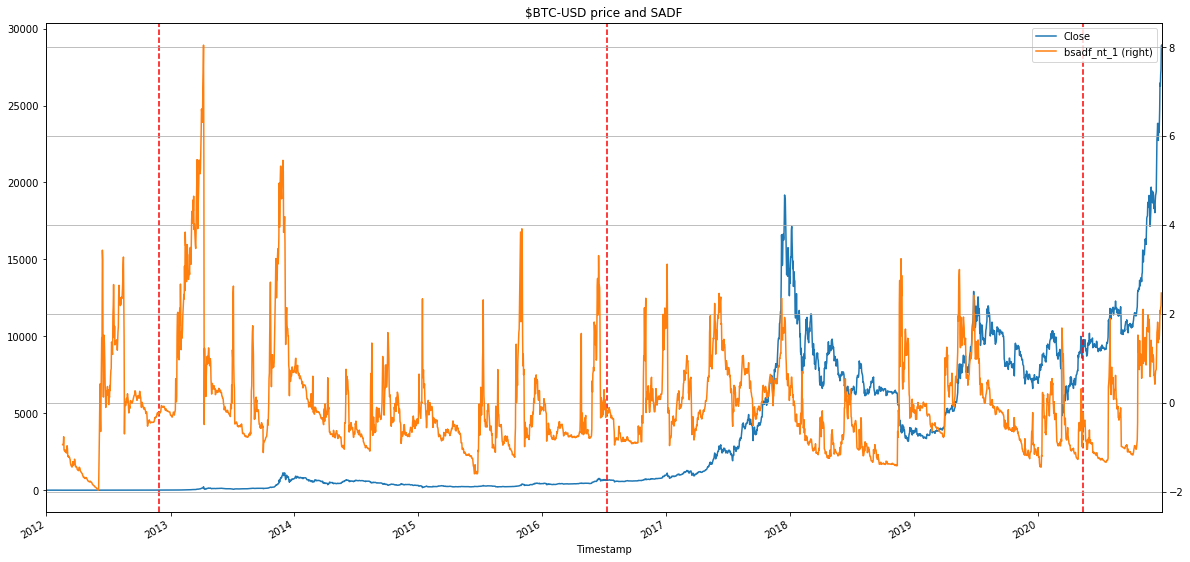
\includegraphics[width=\textwidth]{methods/images/sadf_prices.png}
    \caption{Raw close prices and SADF over time.}
    \label{fig:sadf_prices}
\end{figure}

\begin{figure}[H]
    \centering
    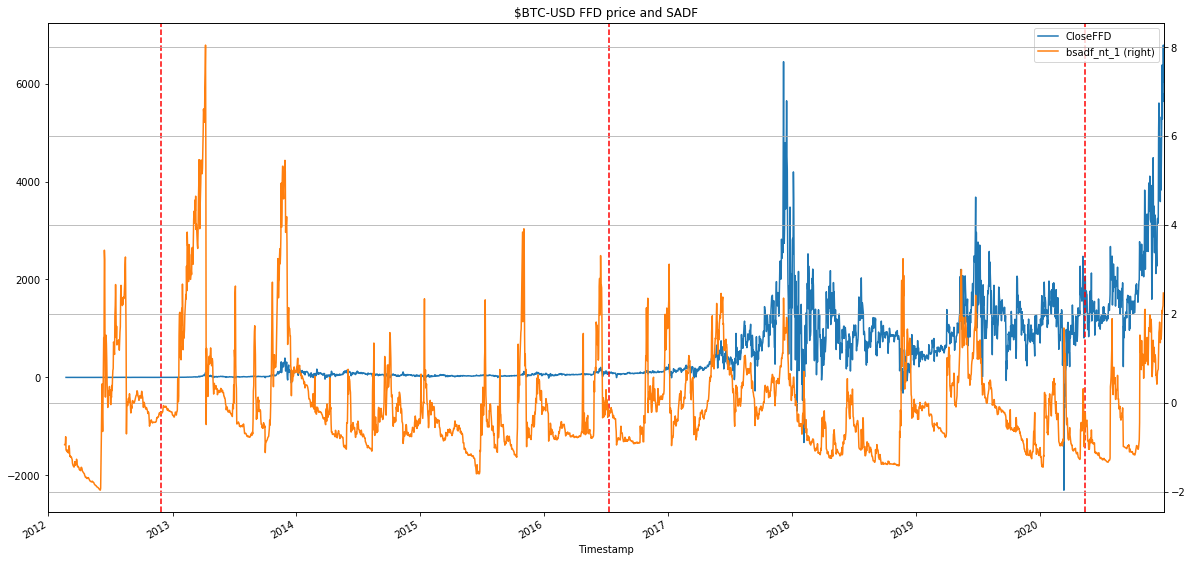
\includegraphics[width=\textwidth]{methods/images/sadf_prices_ffd.png}
    \caption{Fractionally differentiated prices and SADF over time.}
    \label{fig:sadf_prices_ffd}
\end{figure}

\begin{figure}[H]
    \centering
    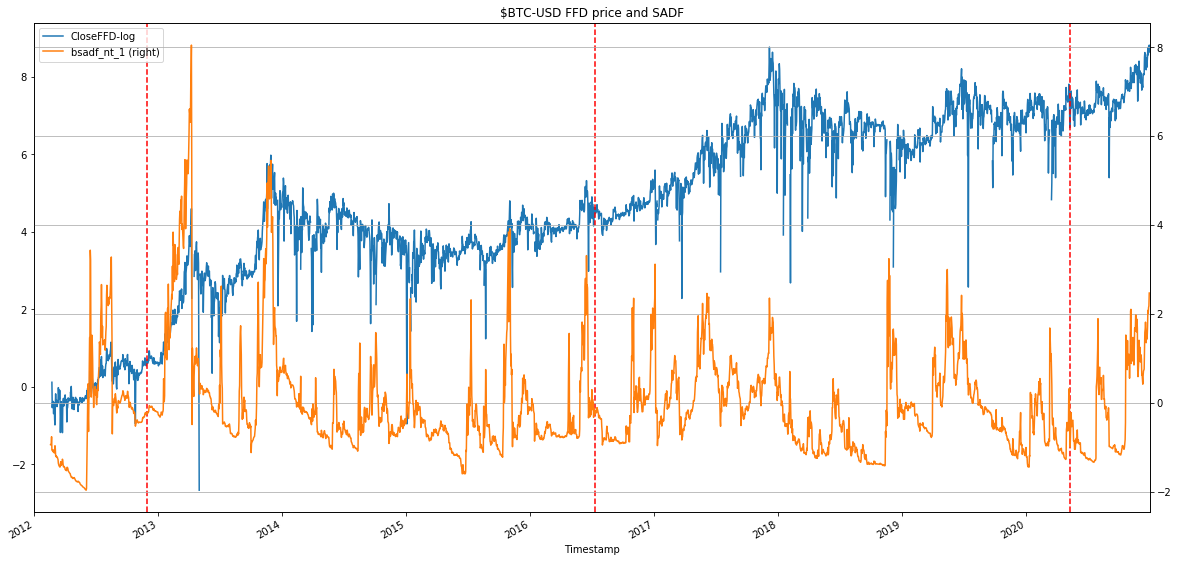
\includegraphics[width=\textwidth]{methods/images/sadf_prices_log.png}
    \caption{Close log-prices and SADF over time.}
    \label{fig:sadf_prices_log}
\end{figure}

